\documentclass[]{tufte-handout}
\usepackage{amsmath,amssymb,amsthm}
\usepackage{tikz}
\usetikzlibrary{arrows}
\usepackage{emp}
\usepackage{ifpdf,graphicx}
\ifpdf
  \DeclareGraphicsRule{*}{mps}{*}{}
\fi
\usepackage{listings}
\usepackage{color}
\usepackage{pdflscape}

\definecolor{dkgreen}{rgb}{0,0.6,0}
\definecolor{gray}{rgb}{0.5,0.5,0.5}
\definecolor{mauve}{rgb}{0.58,0,0.82}

\lstset{frame=tb,
  language=Java,
  aboveskip=3mm,
  belowskip=3mm,
  showstringspaces=false,
  columns=flexible,
  basicstyle={\small\ttfamily},
  numbers=none,
  numberstyle=\tiny\color{gray},
  keywordstyle=\color{blue},
  commentstyle=\color{dkgreen},
  stringstyle=\color{mauve},
  breaklines=true,
  breakatwhitespace=true,
  tabsize=3
}

\empprelude{input metauml}

\tikzset{
  treenode/.style = {align=center, inner sep=0pt, text centered,
    font=\sffamily},
  nd/.style = {treenode, circle, white, font=\sffamily\bfseries, draw=black,
    fill=black, text width=2.5em},% black with white text
  mt/.style = {treenode, rectangle, draw=black,
    minimum width=0.5em, minimum height=0.5em}% mt node (box)
}

\newtheorem{proposition}{Proposition}
 
\title{COMP 210 - Lecture Notes - 08 - Binary Trees, Heaps, and Priority Queues}

\begin{document}
\maketitle

\begin{abstract}
I these notes we look at Binary Trees and related data structures.
\end{abstract}

\section{Binary Trees}

Imagine a list.  Now instead of every non-empty list having a single \textit{next} list, what would happen if you allowed two nexts? What you'd have is a binary tree like the one seen in figure \ref{fig:bintree}. 

\begin{figure}[!htbp]
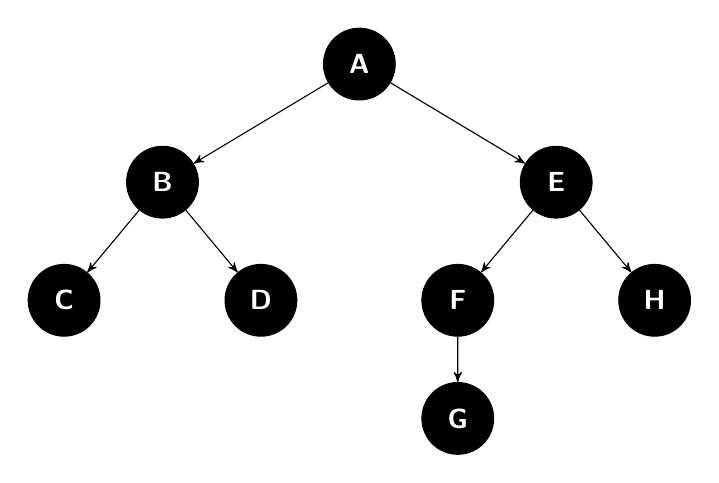
\begin{tikzpicture}[->,>=stealth',level/.style={sibling distance = 5cm/#1,level distance = 1.5cm}] 
\node [nd] {A}
	child{
		node [nd] {B}
			child{ node [nd] {C} }
			child{ node [nd] {D} }
	}
	child{
		node [nd] {E}
			child{
				node [nd] {F} 
					child{ node [nd] {G} } 
			}
			child{ node [nd] {H} }
	}  
;
\end{tikzpicture}
\caption{A Binary Tree}
\label{fig:bintree}
\end{figure}

Great. Let's define this kind of structure using a PDA. If we keep the natural base case of an empty tree then we get a simple extension of a list.  

\begin{empfile}["ln8-bintree"]
\begin{figure*}[ht!]
\begin{emp}(0,0)

Interface.bt("BinTree")
();
classStereotypes.bt("<<interface>>");

Class.mt("MTBinTree")
()
();

Class.node("BinTreeNode")
("-root : Foo","-left : BinTree","-right : BinTree")
();

Class.obj("Foo")
()();

mt.ne = bt.sw + (-10,-30);
node.nw = bt.se + (10,-30);
leftToRight(20)(node,obj);
drawObjects(bt,mt,node,obj);

link(inheritance)(mt.n -- bt.s);
link(inheritance)(node.n -- bt.s);
link(associationUni)(node.n -- bt.se);
link(associationUni)(node.e -- obj.w);

\end{emp}
\caption{A Binary Tree of Foo Objects}
\label{fig:ln8btreePDA}
\end{figure*}
\end{empfile} 

If we wanted, we could then redraw our example tree to show the empty trees as shown in figure \ref{fig:bintree2}. This new diagarm gives us a pretty good feel for the actual structure of a BinTree object where the previous diagram\sidenote{figure \ref{fig:bintree}} highlighted the logical structure of the tree. 

\begin{figure}[!htbp]
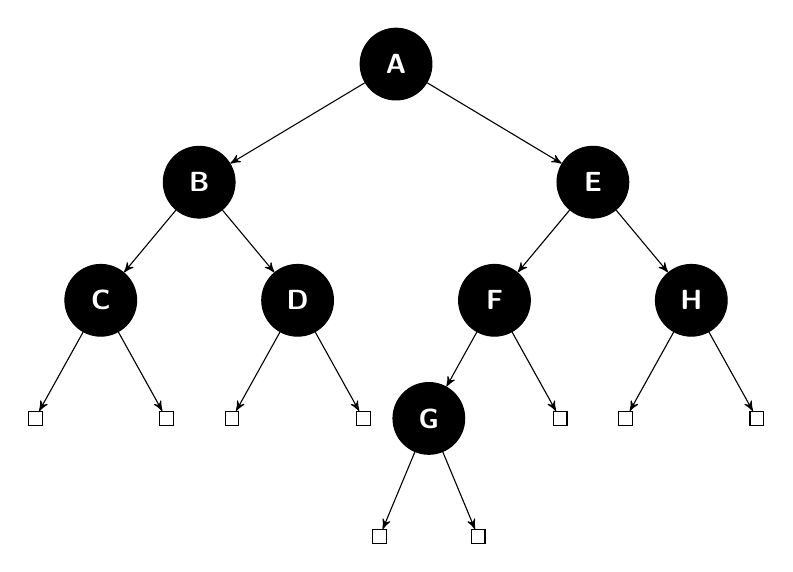
\begin{tikzpicture}[->,>=stealth',level/.style={sibling distance = 5cm/#1,level distance = 1.5cm}] 
\node [nd] {A}
	child{
		node [nd] {B}
			child{ node [nd] {C} 
				child{ node [mt] {} }
				child{ node [mt] {} }
			}
			child{ node [nd] {D} 
				child{ node [mt] {} }
				child{ node [mt] {} }			
			}
	}
	child{
		node [nd] {E}
			child{
				node [nd] {F} 
					child{ node [nd] {G} 
						child{ node [mt] {} }
						child{ node [mt] {} }					
					}
					child{ node [mt] {} }										
			}
			child{ node [nd] {H} 
				child{ node [mt] {} }
				child{ node [mt] {} }					
			}
	}  
;
\end{tikzpicture}
\caption{A Binary Tree with Empty Trees shown}
\label{fig:bintree2}
\end{figure}

It makes sense that the explosion of ``nexts'' leads to an explosion of empty trees. It's often convenient to work with another base case, the singleton tree. There's no reason we can't have two base cases, so let's add this variant of a binary tree to our previous design. The new PDA design given in figure \ref{fig:ln8btreePDA-sing} allows both empty an singleton base cases. It's not yet clear if this is helpful or just extra work, but just drawing simple diagrams shows this might be a nice capability to have as the tree given in figure \ref{fig:bintree3} both covers the complete structure and minimizes the need for a large number of empty trees.  

\begin{empfile}["ln8-bintree2"]
\begin{figure*}[ht!]
\begin{emp}(0,0)

Interface.bt("BinTree")
();
classStereotypes.bt("<<interface>>");

Class.mt("MTBinTree")
()
();

Class.sing("SingletonTree")
("-root : Foo")
();

Class.node("BinTreeNode")
("-root : Foo","-left : BinTree","-right : BinTree")
();

Class.obj("Foo")
()();

topToBottom(30)(bt,sing);
leftToRight(20)(mt,sing,node);
topToBottom(30)(sing,obj);
drawObjects(bt,mt,node,obj,sing);

link(inheritance)(mt.n -- bt.s);
link(inheritance)(node.n -- bt.s);
link(inheritance)(sing.n -- bt.s);
link(associationUni)(node.n -- bt.se);
link(associationUni)(node.s -- obj.n);
link(associationUni)(sing.s -- obj.n);

\end{emp}
\caption{A Binary Tree of Foo Objects with Two Base Cases}
\label{fig:ln8btreePDA-sing}
\end{figure*}
\end{empfile} 


\begin{figure}[!htbp]
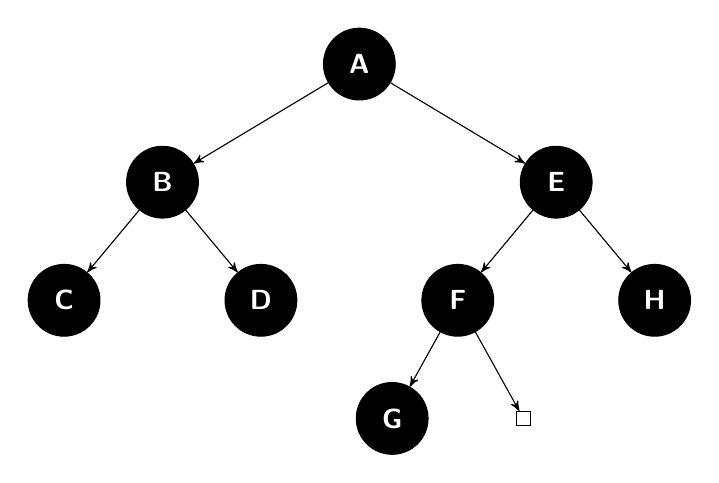
\begin{tikzpicture}[->,>=stealth',level/.style={sibling distance = 5cm/#1,level distance = 1.5cm}] 
\node [nd] {A}
	child{
		node [nd] {B}
			child{ node [nd] {C} }
			child{ node [nd] {D} }
	}
	child{
		node [nd] {E}
			child{
				node [nd] {F} 
					child{ node [nd] {G} }
					child{ node [mt] {} }										
			}
			child{ node [nd] {H} }
	}  
;
\end{tikzpicture}
\caption{A Binary Tree with Empty Trees shown}
\label{fig:bintree3}
\end{figure}

At this point, it's worth imagining how the tree shown in figure \ref{fig:bintree3} might be constructed in Java. For the sake of simplicity, we'll just assume the letters in each circle correspond to the name of some Foo variable.
\begin{figure}[!htpb]
\begin{lstlisting}
BinTree atree = 
	new BinTreeNode( A , 
		new BinTreeNode( B , new SingletonTree(C), new SingletonTree(D)),
		new BinTreeNode( E , 
			new BinTreeNode(F, new SingletonTree(G), new MTBinTree()),
		    new SingletonTree(H))
		); 
\end{lstlisting}
\caption{The tree in figure \ref{fig:bintree3} as a Java BinTree}
\end{figure}

So we have some foothold into the world of trees now. We can define them as recursive class hierarchy and could easily start implementing functionality for that hierarchy so that we could play around with Binary Trees. Before we do that we really should first look at trees in a much broader context and find something interesting to do with trees.

\subsection{Binary Tree Traversal}

Traversing a list is fairly straight forward. From the recursive perspective you either recurse on the rest then deal with the first or your deal with the first then recurse on the rest. If we were computing the size of a list that might look like the snippets we see in figure \ref{fig:lstTrav}. 

\begin{figure}[!htbp]
\begin{lstlisting}

// first, then rest
return 1 + this.rst.size();

// rest, then first
return this.rst.size() + 1;

\end{lstlisting}
\caption{ Recursive List Traversal for \textit{size} }
\label{fig:lstTrav}
\end{figure}

To generalize these patterns we talk about what we do for the first as \textit{visiting} the current node of the list. A little analysis shows that visiting then recursing will visit nodes in first to last order while recurse then visit will visit in last to first. 

With trees we don't just have one recursively defined field but two: the left and right. What are we to do? The answer is simple, pick a permutation of visit (v), go left (l), and go right (r). There are six such permutations: vlr, lvr, lrv, vrl, rvl, and rlv. To simplify matters we only consider permutations where l comes before r. This leaves us with the three \textsc{depth first} traversal patterns. 
\begin{enumerate}
\item \textsc{Preorder Traversal}:  v l r 
\item \textsc{Inorder Traversal}:  l v r
\item \textsc{Postorder Traversal}:  l r v
\end{enumerate}
The names are derived from the placement of the visit within the permutation. In figure \ref{fig:btTrav} we see how each of these patterns could be used to find the size\sidenote{number of non-empty nodes} in a tree.

\begin{figure}[!htbp]
\begin{lstlisting}

// preorder
return 1 + this.left.size() + this.right.size();

// inorder
return this.left.size() + 1 + this.right.size();

//postorder 
return this.left.size() + this.right.size() + 1;

\end{lstlisting}
\caption{ Recursive Binary Tree Traversal for \textit{size} }
\label{fig:btTrav}
\end{figure}

If you wanted to carry these processes out using an iterative loop then you'd need the assistance of a data structure that you studied in COMP220\sidenote{a stack}.  We'll save that task for another time. Right now it's more important to understand the order in which we'll visit a tree's nodes when doing each traversal. For our example tree from figure \ref{fig:bintree3} we'd do the visit orders shown in table \ref{tab:bt3-travs}.

\begin{table}
\begin{tabular}{ll}
\underline{Pattern} & \underline{Visit Order} \\ \\
Preorder (vlr) & A B C D E F G H \\ \\
Inorder (lvr) & C B D A G F E H \\  \\
Postorder (lrv) & C D B A G F H E 
\end{tabular}
\caption{Traversal orders for the tree in figure \ref{fig:bintree3}}
\label{tab:bt3-travs}
\end{table}

Doing these traversals by hand is wonderful practice for thinking through recursive a process. Just like some problems with lists necessitate a last to first traversal and some first to last, there will be tree problems that require different orders for visiting. 

\section{Talking Trees} 

Trees have been studied in mathematics for a long time and have found use in computing for as long as there has been computing.  This means there is a lot of terminology to go along with trees. Much of it pulls from one of two metaphors, family trees or trees in nature.
\begin{itemize}
\item \textbf{Tree Structure}
\begin{itemize}
\item \textsc{Node} A non-empty tree structure containing a single element and a left and right \textit{subtree}. 
\item \textsc{Edge} The connection between a Node and one of its subtrees. 
\item \textsc{Path} A linearly connected set of nodes \\
In our example tree, there is a path from the node containing A to the node containing G through the nodes E and F.
\item \textsc{Root Node} The Root node of a tree is the ``first'' node in that tree. \\
 A is the root of the tree shown in figure \ref{fig:bintree3}. It's left subtree is rooted by the node containing B and its right subtree is rooted by the node containing E.
\item \textsc{Child Node} The root node of a node's subtree.  \\
The node containing B is a child of the node containing A. Children of children and further down are called \textit{descendents}.  The node containing G is a descendent of the node containing E but the node containing D is not a descendent of the node containing E. 
\item \textsc{Parent Node} The node of which a given node is a child. \\
The node containing A is the parent of the node containing B. Notice \textit{the} root of a tree has no parent. Parents of parents and so on up the tree are called \textit{ancestors}. The node containing E is an ancestor of the node containing G but not of the node containing D.
\item \textsc{Leaf Node} A node with no children \\
These nodes are the bottom most layer of a tree. They're what we call the singleton tree and an alternate base case to the empty tree. The nodes containing C, D, G, and H are all leaf nodes. All other nodes are \textit{internal} nodes because they have at least one child.
\end{itemize}
\item \textbf{Properties of Trees and Nodes}
\begin{itemize}
\item \textsc{Node Depth} The number of edges from a given node to the tree's root node. \\
\textit{The} root of a tree always has a depth of 0 and from there depth increases by one with each level. 
\item \textsc{Node Height} The number of edges on the longest path from a give node to a leaf node.
\item \textsc{Tree Height} The height of the tree's root node. \\
This property is the tree analog of list length.
\item \textsc{Tree Size} The number of nodes in the tree. \\
Our example tree has a size of 8.
\end{itemize}
\item \textbf{Classes of Binary Trees}
\begin{itemize}
\item \textsc{(Height) Balanced Binary Tree} A tree in which the height of the left subtree and the height of the right subtree differ by at most one. \\
Our example tree given in figure \ref{fig:bintree3} is height balanced because the left subtree has a height of 1 and the right subtree has a height of 2. 
\item \textsc{Complete Binary Tree} A tree of height $h$ where the tree is full up to depth $h-1$ and then at depth $h$ the leaves fill in from left to right. \\
Complete trees are height balanced.
\item \textsc{Full Binary Tree} A tree where every node except leaf nodes has exactly two children. //
Full trees a special sub-class of Complete trees where every node at depth $h-1$ has two children.
\end{itemize}
\end{itemize}

We've seen a height balanced tree already. Figure \ref{fig:complete} shows you a complete tree of height 2 and figure \ref{fig:full} shows you a full tree of height 2. 

\begin{figure}[!htbp]
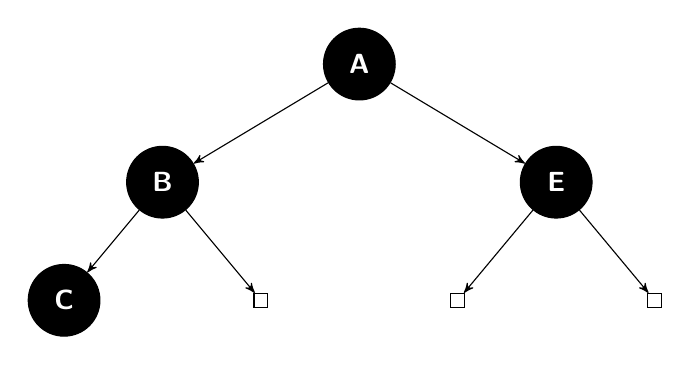
\begin{tikzpicture}[->,>=stealth',level/.style={sibling distance = 5cm/#1,level distance = 1.5cm}] 
\node [nd] {A}
	child{
		node [nd] {B}
			child{ node [nd] {C} }
			child{ node [mt] {} }
	}
	child{
		node [nd] {E}
			child{ node [mt] {} }
			child{ node [mt] {} }													
	}  
;
\end{tikzpicture}
\caption{A Complete Binary Tree of height 2}
\label{fig:complete}
\end{figure}


\begin{figure}[!htbp]
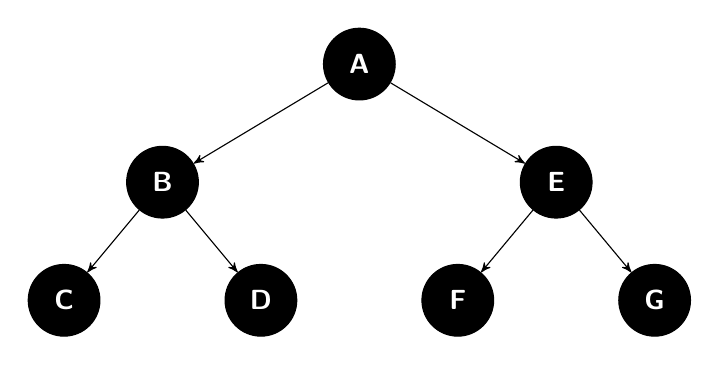
\begin{tikzpicture}[->,>=stealth',level/.style={sibling distance = 5cm/#1,level distance = 1.5cm}] 
\node [nd] {A}
	child{
		node [nd] {B}
			child{ node [nd] {C} }
			child{ node [nd] {D} }
	}
	child{
		node [nd] {E}
			child{ node [nd] {F} }
			child{ node [nd] {G} }													
	}  
;
\end{tikzpicture}
\caption{A Full Binary Tree of height 2}
\label{fig:full}
\end{figure}

Now we know how to talk about trees, but what do we do with them? 

\section{An Application of Trees: Codes}

Let's say you send a letter to your friend and it's 10,000 characters long. If this letter is encoded in ASCII or UTF-8, then each character requires 1 Byte to encode and the letter clocks in at 10kB\sidenote{assuming its plain text of course}. Could we do better in terms of message size?  

One option would be to define another fixed length encoding scheme that uses fewer than 8 bits per character. If your letter uses $N <= 2^n$ characters with $n < 8$ then you could simply devise your own scheme using that number of bits. Another option would be variable length encoding.  Basic engineering tells us to optimize the common case. If we could devise a code system where highly frequent characters had shorter codes then we might be able to do even better. Given that natural language character frequencies are far from uniform, we have high hopes that our letter has a really nice variable length encoding scheme. 

Variable length encoding schemes have a few problems not the least of which is figuring out where one letter stops and one starts without doing some costly computation.\sidenote{Fixed length codes do not suffer this problem. You simply read in fixed sized increments}. To avoid this problem we need a \textit{prefix free code}. In prefix free codes, no one code is a prefix for another code.  For example, if $010$ is the code for \textit{a}, then $010$ cannot occur at the start of any other character code. If we guarantee this property then reading encoded messages is unambiguous.  If you read $0$ then $1$ then $0$ you must have just read \textit{a} because no other code could possibly start that way. A prefix free code could have variable code lengths for each character and seems to provide a means of solving the where one character ends and another begins problem. So, let's look at the problem of how one generates such a code before we worry about the compression part. 

I'll begin with what seems like an obvious statement about binary tree paths. Take a moment to convince yourself that it must be true\sidenote{bonus if you prove it mathematically}.
\begin{quote}
The path from a tree's root node to one of its leaf nodes is not a sub-path for any other path in the tree. 
\end{quote}
Given that each path terminates at the leaf, then no other paths follow the leaf and the path to the leaf is obviously not a subpath for something else. Now what if paths somehow represented character codes? Then sub-paths must be prefixes and this statement is equivalent to saying:
\begin{quote}
The code represented by a path from the root to a leaf node is not the prefix of another other code.  
\end{quote}
To turn this into a workable coding system we simply place our characters in the leaves of a tree. Codes are then formed by starting at the root of the tree, reading a $0$ each time we go left and a $1$ when we go right\sidenote{or the other way around}. When a leaf is reached then the binary code we've read is the code for that character. Let's say we had three letters: a, b, and c. One possible variable length, prefix free code for this alphabet would be represented with the tree given in figure \ref{fig:abc-var}.

\begin{figure}[!htbp]
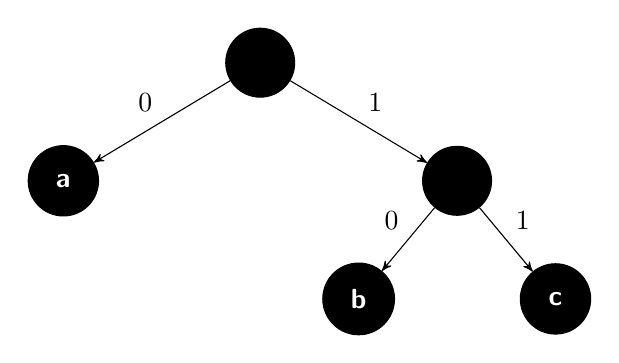
\begin{tikzpicture}[->,>=stealth',level/.style={sibling distance = 5cm/#1,level distance = 1.5cm}] 
\node [nd] {}
	child{ node [nd] {a} edge from parent node[above left] {0} }                         
	child{ node [nd] {} 
			child{ node [nd] {b} edge from parent node[above left] {0} }													
			child{ node [nd] {c} edge from parent node[above right] {1} }									
			edge from parent node[above right] {1} 
	}				
;
\end{tikzpicture}
\caption{Code as Tree. a = 0, b = 10, c = 11.}
\label{fig:abc-var}
\end{figure}

We've now reduced prefix-free code production to a simple binary tree construction problem.  The trick is to construct the \textit{right} tree. Clearly there are lots of different trees we could construct for any given alphabet. In fact, we can even make a fixed length code from a tree. Figure \ref{fig:abc-fix} gives a code-as-tree encoding of a fixed length code for our a, b, and c alphabet.\sidenote{In fact, figure \ref{fig:abc-var} implies that ASCII can be represented by a tree of height 8. Do you see how?}.

\begin{figure}[!htbp]
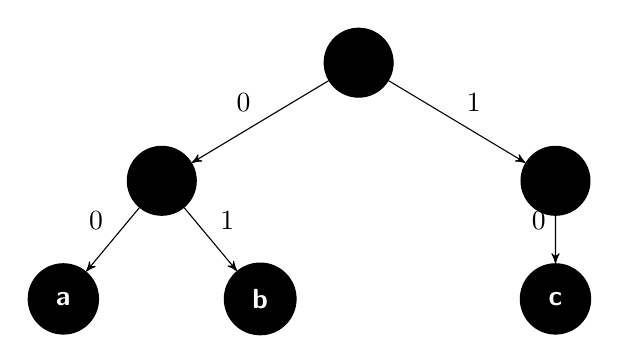
\begin{tikzpicture}[->,>=stealth',level/.style={sibling distance = 5cm/#1,level distance = 1.5cm}] 
\node [nd] {}
	child{ node [nd] {} 
			child{ node [nd] {a} edge from parent node[above left] {0} }													
			child{ node [nd] {b} edge from parent node[above right] {1} }									
			edge from parent node[above left] {0} }                         
	child{ node [nd] {} 
			child{ node [nd] {c} edge from parent node[above left] {0} }													
			edge from parent node[above right] {1} 
	}				
;
\end{tikzpicture}
\caption{Code as Tree. a = 00, b = 01, c = 10.}
\label{fig:abc-fix}
\end{figure}

Let's step back a second now. Fixed length codes correspond to complete or full binary trees. What about variable length prefix-free codes? It's hard to say as they seem much more flexible. However, if our goal is short code lengths then what we might be looking for is something balanced and shallow or at least just shallow. 

\subsection{Huffman Codes}

David Huffman devised a method to construct variable length, prefix free codes that minimized the length of the encoded message and proved that his code was optimal for all such codes \cite{huff}. What Huffman did was effectively construct a tree based on the probability of each character from the alphabet occurring. For compressing a single message we can swap out relative frequencies for probabilities and get maximal compression for that document. 

The tree that results from Huffman's algorithm is called a \textit{Huffman Tree}.  It's pretty much the exact kind of tree-based representation of a code we looked at before but adjusted to support the algorithm for constructing it. 
\begin{itemize}
\item Leaf nodes represent letters
\item All nodes have a numerical weight associated with them. For leaf nodes, that weight is the probability/relative frequency of the letter it represents. For non-leaf nodes, the weight is the sum of the weights of its subtress. 
\end{itemize}  
Huffman's algorithm employs a greedy strategy. We begin with the collection of all the leaf nodes. We then repeat the following process until the collection contains a single tree: remove the two least weighted trees, construct a new tree with these threes as the subtrees, and insert that tree back into the collection. The tree that results is the Huffman tree for your code. 

Let's do toy example before we go further. Table \ref{tab:huff-ex} lists a simple three letter alphabet and the relative frequency of each letter. 
\begin{table}
\begin{tabular}{cc}
\underline{letter} & \underline{frequency} \\ 
a & .38 \\
b & .05 \\
c & .57 
\end{tabular}
\label{tab:huff-ex}
\caption{A simple three letter alphabet with frequencies}
\end{table}

The formation of a Huffman Tree for our toy alphabet is shown in figure \ref{fig:huff-ex-0}. The algorithm requires two iterations of Huffman's process to complete.  

\begin{figure}[!htbp]

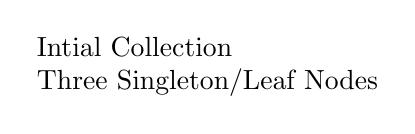
\begin{tikzpicture}[->,>=stealth',level/.style={sibling distance = 5cm/#1,level distance = 1.5cm}] 
\node[align=left] {Intial Collection \\ Three Singleton/Leaf Nodes};
\end{tikzpicture}%
\hspace{.25in}%
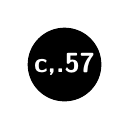
\begin{tikzpicture}[->,>=stealth',level/.style={sibling distance = 5cm/#1,level distance = 1.5cm}] 
\node [nd] {c,.57};
\end{tikzpicture}%
\qquad%
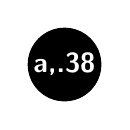
\begin{tikzpicture}[->,>=stealth',level/.style={sibling distance = 5cm/#1,level distance = 1.5cm}] 
\node [nd] {a,.38};
\end{tikzpicture}%
\qquad%
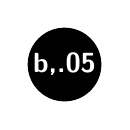
\begin{tikzpicture}[->,>=stealth',level/.style={sibling distance = 5cm/#1,level distance = 1.5cm}] 
\node [nd] {b,.05};
\end{tikzpicture}

\vspace{.25in}

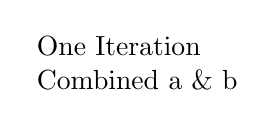
\begin{tikzpicture}[->,>=stealth',level/.style={sibling distance = 5cm/#1,level distance = 1.5cm}] 
\node[align=left] {One Iteration \\ Combined a \& b };
\end{tikzpicture}%
\hspace{.25in}%
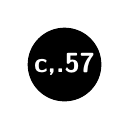
\begin{tikzpicture}[->,>=stealth',level/.style={sibling distance = 5cm/#1,level distance = 1.5cm}] 
\node [nd] {c,.57};
\end{tikzpicture}%
\qquad%
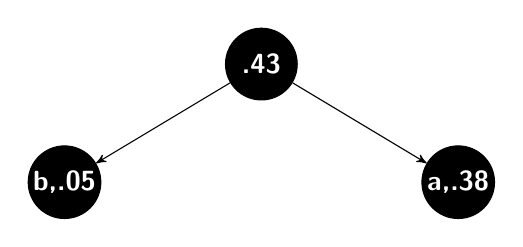
\begin{tikzpicture}[->,>=stealth',level/.style={sibling distance = 5cm/#1,level distance = 1.5cm}] 
\node [nd] {.43}
	child{ node [nd] {b,.05}  }
	child{ node [nd] {a,.38}  }
;
\end{tikzpicture}

\vspace{.25in}

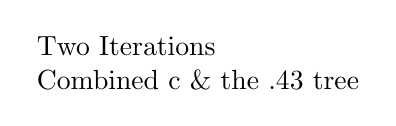
\begin{tikzpicture}[->,>=stealth',level/.style={sibling distance = 5cm/#1,level distance = 1.5cm}] 
\node[align=left] {Two Iterations \\ Combined c \& the .43 tree};
\end{tikzpicture}%
\hspace{.25in}%
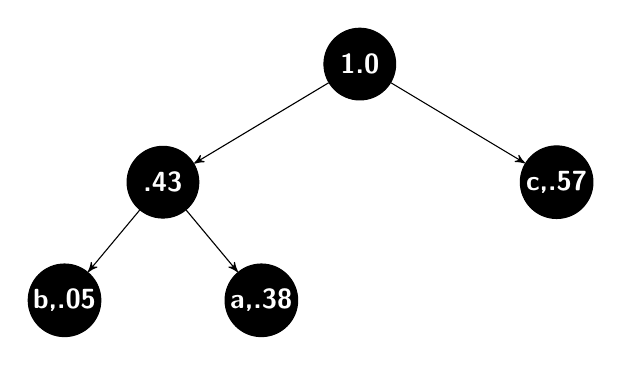
\begin{tikzpicture}[->,>=stealth',level/.style={sibling distance = 5cm/#1,level distance = 1.5cm}] 
\node [nd] {1.0}
	child{ node [nd] {.43}
		child{ node [nd] {b,.05}  }
		child{ node [nd] {a,.38}  }
	}
	child{ node [nd] {c,.57} }
;
\end{tikzpicture}

\caption{Huffman's Algorithm Example}
\label{fig:huff-ex-0}
\end{figure}

The code produced by this tree is given in table \ref{tab:huffcodes}.
\begin{table}
\begin{tabular}{cc}
\underline{letter} & \underline{code} \\ 
a &  01 \\
b &  00 \\
c &  1
\end{tabular}
\label{tab:huffcodes}
\caption{A Huffman code for the simple three letter alphabet given in table \ref{tab:huff-ex}}
\end{table}

Huffman proved that his code is optimal, that it minimizes the expected length of the message it's encoding compared to any code that existed at the time and that will ever exist. What's clear is that path length is important and that the shorter the path the better. Thus, if we start understand general relationships between the number of nodes or leaves and a tree and potential tree heights we can start to get a better understand of how and why trees are useful in solving problems. 

\section{Structure and Its Implications}

Looking at coding, Huffman codes, and trees has shown us that trees can help us solve problems by embedding problem logic in the structure of a tree.  It follows then that understanding certain properties of tree structures lets us understand properties of the process/problem represented by that tree. Much of what we need or want to know boils down to questions relative to size and height. For example, if you want to know the minimum length of a fixed length code for an alphabet with $n$ symbols then you could just figure out the minimum height possible for a tree with $n$ leaves. This leads to a series of questions about the relationships between size, number of leaves, and height.
\begin{enumerate}
\item What's the min height for a tree with $n$ leaves? What's the min/max number of internal nodes for such a tree?
\item How many nodes can a tree of height $h$ contain? How many leaves?
\item What's the min/max path length for a tree containing $n$ nodes? What about $n$ leaves? 
\end{enumerate}

Let's begin with a constrained version of one of the more basic questions: \textit{how many leaves are on a \textit{full} tree of height $h$?}. This question sets some very useful bounds on the number of leaves as full trees maximize leaves relative to height\sidenote{can you see why? could you prove it?}. To make things easy we'll start with the trivial cases and work up for a bit to find a pattern. The super-trivial case is the empty tree: there are no leaves on an empty tree nor does an empty tree have any height to speak of. A tree of height 0 is just a singleton and it is trivially a leaf. To increase the height to 1 and keep the tree full we add two children to that one node and get 2 leaves.  For height 2 we add two children to each of those nodes obtaining 4 leaves. All these trees are shown in figure \ref{fig:full012}.

\begin{figure}
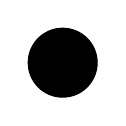
\begin{tikzpicture}[->,>=stealth',level/.style={sibling distance = 5cm/#1,level distance = 1.5cm}] 
\node [nd] {};
\end{tikzpicture}%
\qquad%
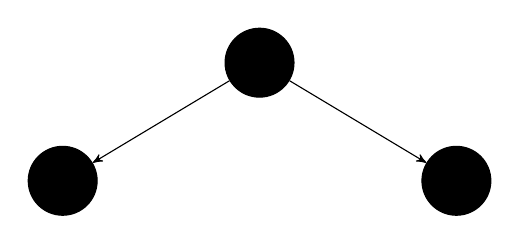
\begin{tikzpicture}[->,>=stealth',level/.style={sibling distance = 5cm/#1,level distance = 1.5cm}] 
\node [nd] {}
	child{ node [nd] {} }
	child{ node [nd] {} }
;
\end{tikzpicture}%
\qquad%
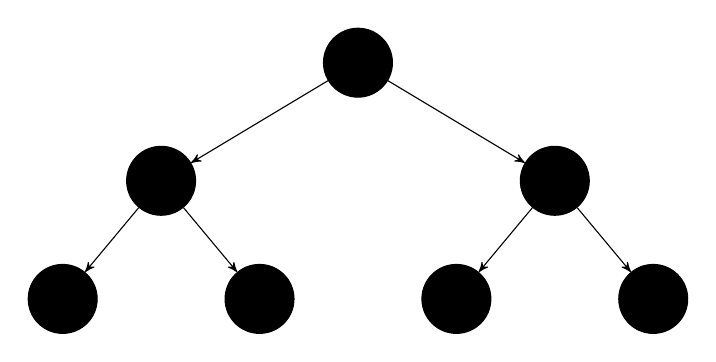
\begin{tikzpicture}[->,>=stealth',level/.style={sibling distance = 5cm/#1,level distance = 1.5cm}] 
\node [nd] {}
	child{ node [nd] {} 
		child{ node [nd] {} }
		child{ node [nd] {} }	
	}
	child{ node [nd] {} 
		child{ node [nd] {} }
		child{ node [nd] {} }	
	}
;
\end{tikzpicture}
\caption{Full Trees of height 0, 1, and 2}
\label{fig:full012}
\end{figure}

The doubling of leaves is clearly going to continue and the underlying pattern is the familiar powers of 2. Now what about size? What's the size of these trees? Again, let's just count up from simple cases and see if we see a pattern. The singleton tree is obviously size 1. A full tree of height 1 is the root and two children, so 3. Next, for height 2 we add to that three 4 children for a size of 7. At height 3 we add 8 children to the 7 nodes of the height 2 full tree for a total of  15 nodes. Do you see the pattern? What if you added 1 to each of these numbers? You have $\{2,4,8,16\}$. The size seems to be one less than $2^h$. What you just solved intuitively is the following well proposition about a series:

\begin{proposition}
\[\sum\limits_{i=0}^{h} 2^i = 2^{h+1}-1\]
\begin{proof}
The proof follows by induction on $h$. For $h=0$ we see $2^0 = 1$ and $2^{1}-1= 1$ so the base case holds. We now prove that if $\sum\limits_{i=0}^{k} 2^i = 2^{k+1}-1$ for $k\geq0$, then it will also be true for $k+1$. 
\begin{equation*}
\begin{array}{lcr}
\sum\limits_{i=0}^{k+1} 2^i &=& 2^{k+1} + \sum\limits_{i=0}^{k} 2^i \\ \\
 &=& 2^{k+1} + 2^{k+1} - 1 \\ \\
 &=& 2(2^{k+1}) - 1 \\ \\
  &=& 2^{k+2} - 1 \\ \\
\end{array}
\end{equation*}
This is equivalent to $2^{(k+1)+1}-1$ and so by mathematical induction $\sum\limits_{i=0}^{h} 2^i = 2^{h+1}-1$ for all $h\geq0$.
\end{proof}
\end{proposition}

We now know some important properties about the number of leaves and total nodes for full trees. These are captured in table \ref{tab:fulltrees}.

\begin{table}
\begin{tabular}{ccc}
\underline{height} & \underline{Num. Leaves} & \underline{Size} \\
empty & 0 & 0 \\
0 & 1 & 1\\
1 & 2 & 3\\
2 & 4 & 7\\
3 & 8 & 15\\
$\ldots$ & $\ldots$ & $\ldots$ \\
$h$ & $2^h$ & $2^{h+1}-1$ 
\end{tabular}
\caption{Properties of Full trees}
\label{tab:fulltrees}
\end{table}

From here we can relax our thinking a bit and look at complete trees. For a complete tree of height $h$ there is a full tree of height $h-1$ and one of $h$ that give us lower and upper bounds for leaves and size. Let's just look at all the complete trees of height 2 as shown in figure \ref{fig:complete2}. We exclude from this list the full tree of height 2 as we're interested in trees that are strictly complete and not also full. 

\begin{figure}
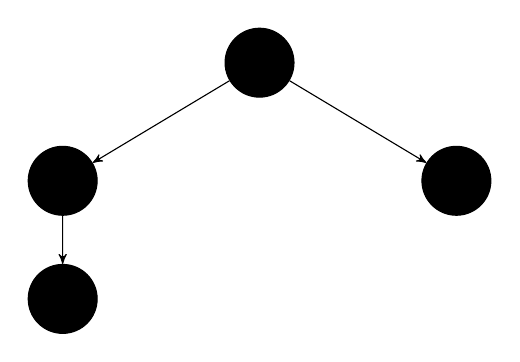
\begin{tikzpicture}[->,>=stealth',level/.style={sibling distance = 5cm/#1,level distance = 1.5cm}] 
\node [nd] {}
	child{ node [nd] {} 
		child{ node [nd] {} }		
	}
	child{ node [nd] {} }
;
\end{tikzpicture}%
\qquad%
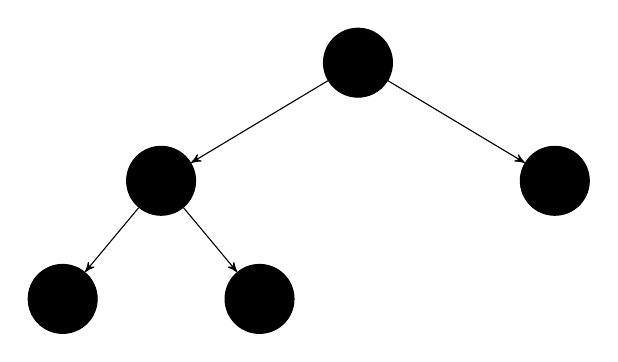
\begin{tikzpicture}[->,>=stealth',level/.style={sibling distance = 5cm/#1,level distance = 1.5cm}] 
\node [nd] {}
	child{ node [nd] {} 
		child{ node [nd] {} }
		child{ node [nd] {} }	
	}
	child{ node [nd] {} }
;
\end{tikzpicture}%
\qquad%
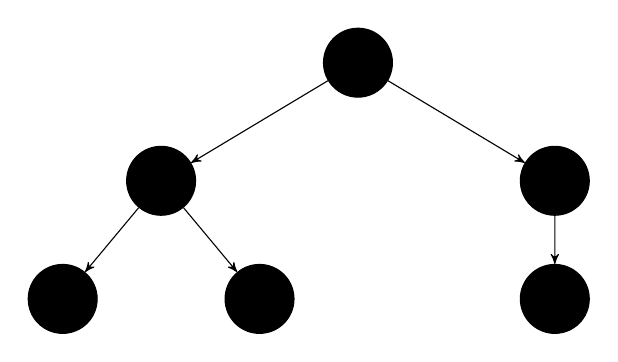
\begin{tikzpicture}[->,>=stealth',level/.style={sibling distance = 5cm/#1,level distance = 1.5cm}] 
\node [nd] {}
	child{ node [nd] {} 
		child{ node [nd] {} }
		child{ node [nd] {} }	
	}
	child{ node [nd] {} 
		child{ node [nd] {} }		
	}
;
\end{tikzpicture}
\caption{All the Complete Trees of height 2}
\label{fig:complete2}
\end{figure}

First lets address the number of leaves question for complete trees. In the minimal case we seem to simply swap one leaf at $h$ for a leaf in the full tree at $h-1$. So the lower bound for number of leaves is $2^{h-1}$ the upper bound has one fewer than the full tree at $h$ so we're looking at $2^{h}-1$. Looking at tree sizes is also straight forward. On the low end we have 1 more node than a full tree at height $h-1$, or $2^{h}$ and on the high end one less node than a full tree at height $h$, or $2^{h+1}-2$.  Finally, it's worth noting that there are no binary trees of height 0 that are full but not complete. 

\begin{table}
\begin{tabular}{ccccc}
\underline{height} & \underline{min leaves} & \underline{max leaves} & \underline{min size} & \underline{max size} \\
1 & 1 & 1 & 2 & 2 \\
2 & 2 & 3 & 4 & 6 \\
3 & 4 & 7 & 8 & 14 \\
$\ldots$ & $\ldots$ & $\ldots$ & $\ldots$ & $\ldots$ \\
$h$ & $2^{h-1}$ & $2^h - 1$ & $2^h$ & $2^{h+1}-2$
\end{tabular}
\caption{Properties of Complete (but not full) tree}
\label{tab:completeprops}
\end{table} 

So why all this fuss over full and complete trees? The full binary tree maximizes size and leaves while minimizing tree height. You cannot have any more nodes in a depth $h$ tree than you do in a full tree. Complete trees do something similar but for height balanced trees. You cannot have any more nodes in a height balanced tree than you do in a complete tree that's one node shy of being full. Now remember that tree height sets the upper bound on path length.  It's the path length that we're often most interested in. Huffman wanted a short expected path length to maximize the compression of the message. In lots of cases we just need a short upper bound on paths.  Understanding the path length properties of complete and full trees thereby lets us some well behaved cases. 

Now we flip all of these problems around. Given a full tree of size $n$, what's the height of the tree. We know that $n$ is exactly $2^{h+1}-1$ so all we need to do is solve for $h$
\begin{equation*}
\begin{array}{rcl}
2^{h+1}-1 &=& n \\
2^{h+1}  &=&  n + 1 \\
\log_2(2^{h+1})  &=&  \log_2(n + 1) \\
h+1 &=& \log_2(n + 1) \\
h &=& \log_2(n + 1)-1 \\
h &=& O(\log n)   
\end{array}
\end{equation*}

It's important to note that for a full tree of $n$ nodes the quantity $n+1$ is an exact power of two so our heights will always come out an exact integer value. Let's just test this with a concrete example. A full tree of height $4$ has $2^{4+1}-1 = 15$ nodes and $\log_2(15+1)-1 = \log_2(16)-1 = 5-1 = 4$. When $n$ is the number of leaves in a full tree then we know $n = 2^h$ and the height is clearly $\log_2 n$. What have we learned? The height of a full tree is on order the logarithm of its size or the number of its leaves. 

What about a complete tree of size $n$? We know $n$ must between $2^h$ and $2^{h+1}-2$. When $n$ is the minimum size, then the height is $\log_2n$, but what about when it's not the minimum? We know for certain that it will not reach the next power of 2 without actually increasing the height of the tree so the simply solution is to simply take the log and round down to the nearest integer, $\lfloor \log_2 n \rfloor$.




\section{Priority Queues, Heaps, and Huffman's Forest}

If my alphabet contains $n$ characters, then I'll need $n-1$ iterations of Huffman's process to get the final Huffman tree. Each iteration selects the minimum tree from the forest twice, constructs a new tree, and inserts that new tree back to the collection. If we want this process to be efficient, then we need those operations to be efficient. It doesn't take much to see that tree construction is take $O(1)$ operations\sidenote{just assign pointers for left and right along with the new root's value}. The real trick\sidenote{it often is} is having efficient operations for our collection. 







\bibliographystyle{plain}
\bibliography{huffcode}
\end{document}
